\documentclass[t]{beamer}
\usepackage[utf8]{inputenc}  % to be able to type unicode text directly
%\usepackage[french]{babel}   % french typographical conventions
\usepackage{inconsolata}     % for a nicer (e.g. non-courier) tt family font
%\usepackage{amsthm,amsmath}  % fancier mathematics
\usepackage{array} % to fine-tune tabular spacing
\usepackage{bbm} % for blackboard 1

\usepackage{graphicx}        % to include images
%\usepackage{animate}         % to include animated images
\usepackage{soul}            % for colored strikethrough
%\usepackage{bbding}          % for Checkmark and XSolidBrush
\usepackage{hyperref,url}

\colorlet{darkgreen}{black!50!green}  % used for page numbers
\definecolor{term}{rgb}{.9,.9,.9}     % used for code insets

\setlength{\parindent}{0em}
\setlength{\parskip}{1em}


% coco's macros
\def\R{\mathbf{R}}
\def\F{\mathcal{F}}
\def\x{\mathbf{x}}
\def\y{\mathbf{y}}
\def\u{\mathbf{u}}
\def\Z{\mathbf{Z}}
\def\d{\mathrm{d}}
\DeclareMathOperator*{\argmin}{arg\,min}
\DeclareMathOperator*{\argmax}{arg\,max}
\newcommand{\reference}[1] {{\scriptsize \color{gray}  #1 }}
\newcommand{\referencep}[1] {{\tiny \color{gray}  #1 }}
\newcommand{\unit}[1] {{\tiny \color{gray}  #1 }}

% disable spacing around verbatim
\usepackage{etoolbox}
\makeatletter\preto{\@verbatim}{\topsep=0pt \partopsep=0pt }\makeatother

% disable headings, set slide numbers in green
\mode<all>\setbeamertemplate{navigation symbols}{}
\defbeamertemplate*{footline}{pagecount}{\leavevmode\hfill\color{darkgreen}
   \insertframenumber{} / \inserttotalframenumber\hspace*{2ex}\vskip0pt}

%% select red color for strikethrough
\makeatletter
\newcommand\SoulColor{%
  \let\set@color\beamerorig@set@color
  \let\reset@color\beamerorig@reset@color}
\makeatother
\newcommand<>{\St}[1]{\only#2{\SoulColor\st{#1}}}
\setstcolor{red}

% make everything monospace
\renewcommand*\familydefault{\ttdefault}

% define a font size tinier than tiny
\makeatletter
\newcommand{\srcsize}{\@setfontsize{\srcsize}{5pt}{5pt}}
\makeatother


\begin{document}

\addtocounter{framenumber}{-1}
\begin{frame}[plain,fragile]
\LARGE\begin{verbatim}





   Kadkhodaie-Simoncelli dynamics




mnhrdt
gtti 1/2/2024
\end{verbatim}
\end{frame}

% recall gaussian noise and gaussian blur
\begin{frame}[noframenumbering]

	\vfill
\begin{center}
{\color{red}\Huge
	WARNING!

	Important distinction:
}
\end{center}
	\vfill

%SCRIPT plambda photos/gbarbsquare.png "randg 40 * +" -o f/gnoise.png
%SCRIPT blur g 10  photos/gbarbsquare.png f/gblur.png

\begin{tabular}{cc}%c}
	%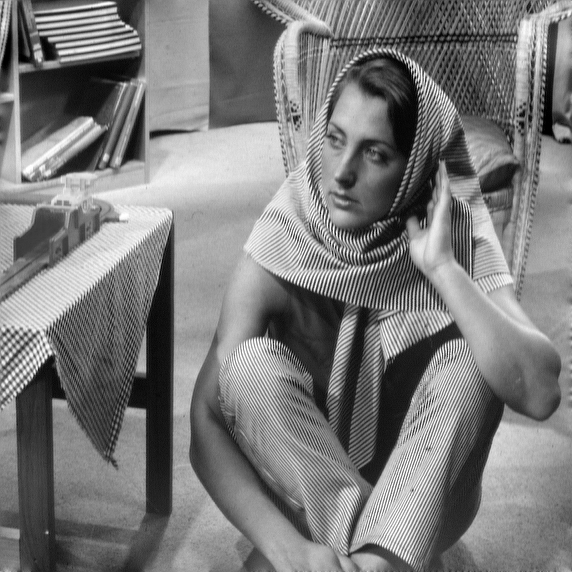
\includegraphics[width=0.3\linewidth]{photos/gbarbsquare.png}&
	\includegraphics[width=0.46\linewidth]{f/gnoise.png}&
	\includegraphics[width=0.46\linewidth]{f/gblur.png}\\
	%input image &
	\color{red} gaussian noise &%$\sigma=30$ &
	\color{red} gaussian blur %/$\sigma=10$ \\
\end{tabular}
	\vfill
\end{frame}




\begin{frame}
CONTEXT: GTTIS ABOUT DIFFUSION MODELS\\
=====================================

\vfill
\begin{columns}
	\begin{column}{0.3\textwidth}\srcsize
		{\bf Valentin de Bortoli},
		{\color{gray} October 2023}\\
		{Diffusion Schrödinger Bridge and Generative Modeling}
		\vspace{4em}

		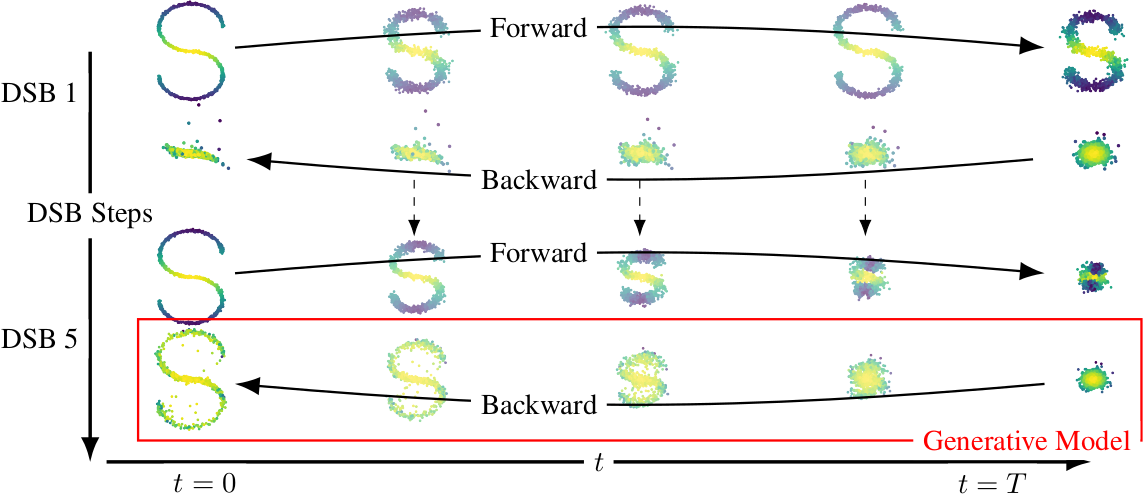
\includegraphics[width=\linewidth]{photos/borto_shot1.png}
		\vspace{4em}

		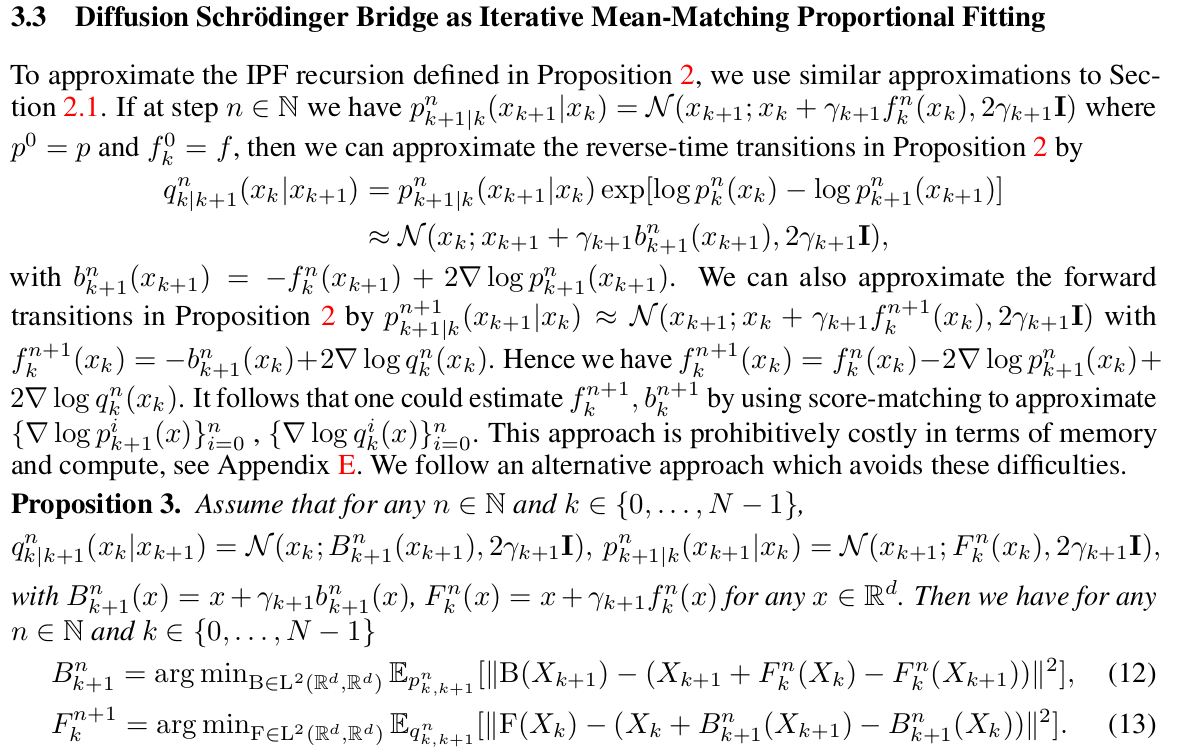
\includegraphics[width=\linewidth]{photos/borto_shot2.png}
	\end{column}
	\pause
	\begin{column}{0.3\textwidth}\srcsize
		{\bf Zhe Zheng},
		{\color{gray} January 2024}\\
		{Denoiser and Its Application Beyond Denoising}
		\vspace{1em}

		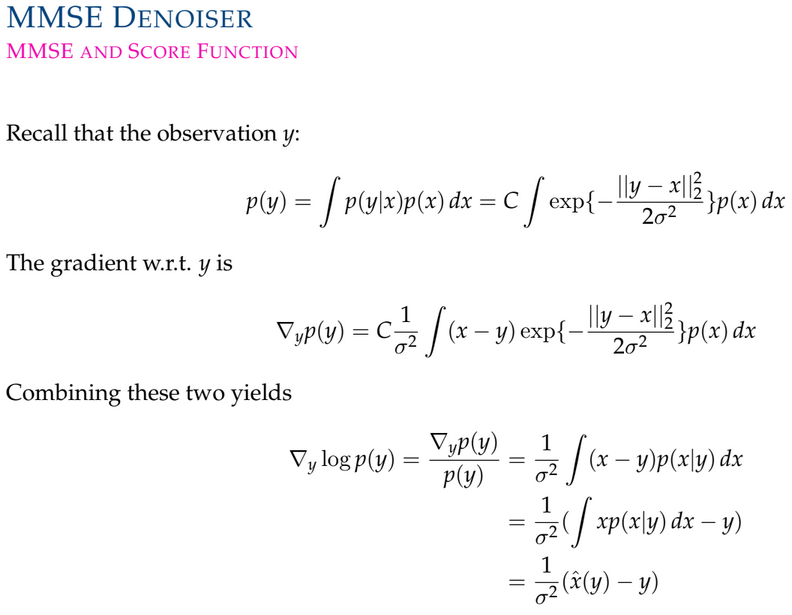
\includegraphics[width=\linewidth]{photos/zhe_shot0.png}
		\vspace{1em}

		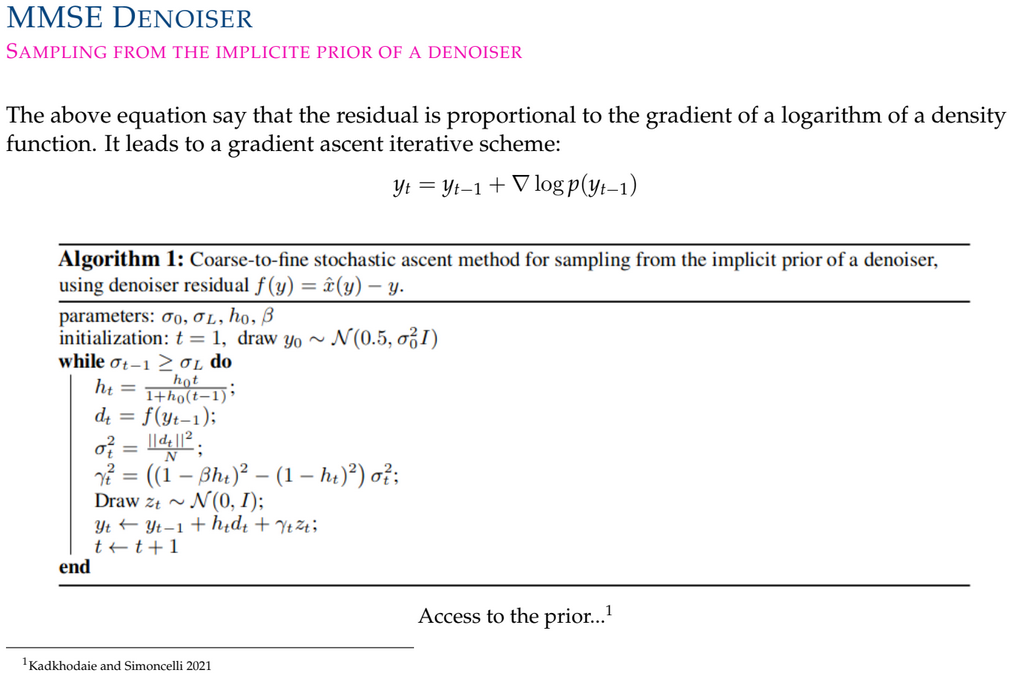
\includegraphics[width=\linewidth]{photos/zhe_shot1.png}
		\vspace{1em}

		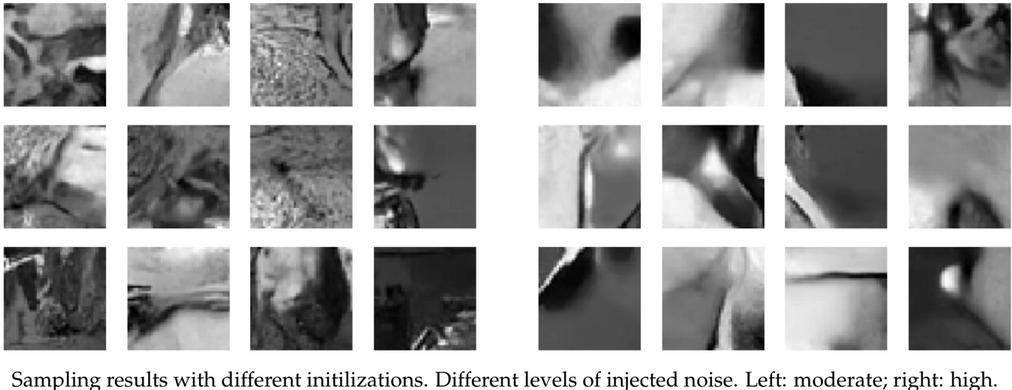
\includegraphics[width=\linewidth]{photos/zhe_shot2.jpg}
	\end{column}
	\pause
	\begin{column}{0.3\textwidth}\srcsize
		{\bf Enric Meinhardt-Llopis},
		{\color{gray} February 2024}\\
		\vspace{4em}

		\pause
		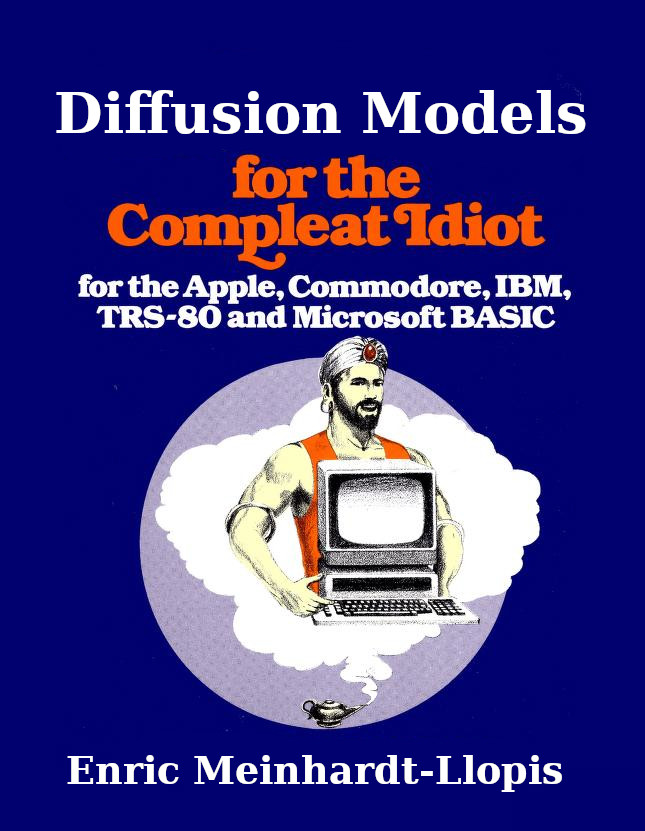
\includegraphics[width=\linewidth]{photos/compleat.jpg}
	\end{column}
\end{columns}
\vfill
\end{frame}

\begin{frame}
CONTEXT: THE BASIC IDEA\\
=======================

\only<1>{
\vfill

\includegraphics[width=\linewidth]{photos/gobrrr.png}
\vfill}\only<2-3>{
	{\scriptsize
{\bf Solving Linear Inverse Problems Using the Prior Implicit in a Denoiser}\\
\vspace{-0.5em}{\color{gray}Kadkhodaie-Simoncelli 2021}
}

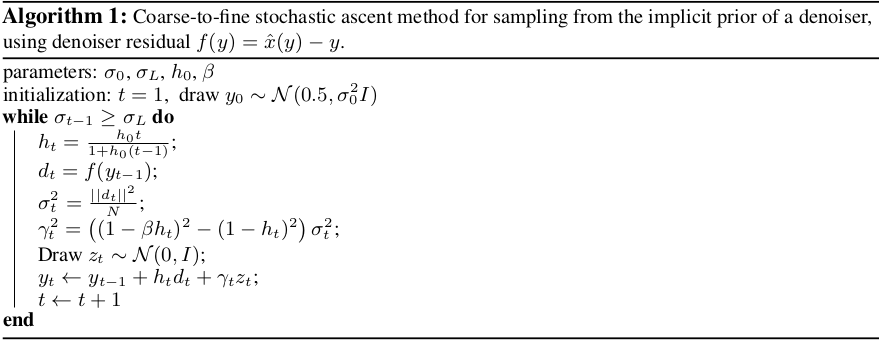
\includegraphics[width=0.9\linewidth]{ks.png}
}\only<3>{
	\vfill
\tiny
\begin{tabular}{lll}
	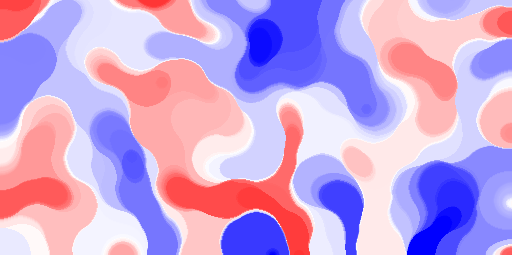
\includegraphics[height=0.18\textheight]{somiters3b.png} &
	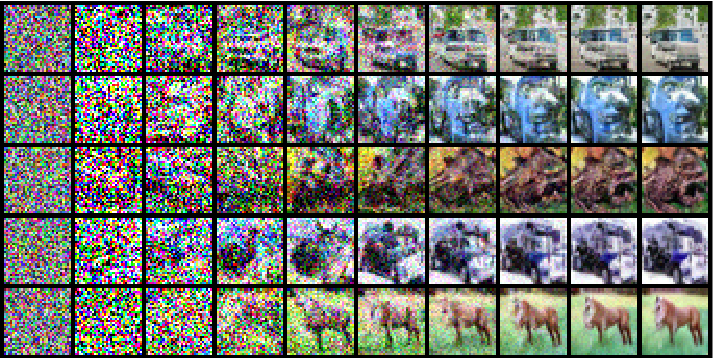
\includegraphics[height=0.18\textheight]{songermon1b.png} &
	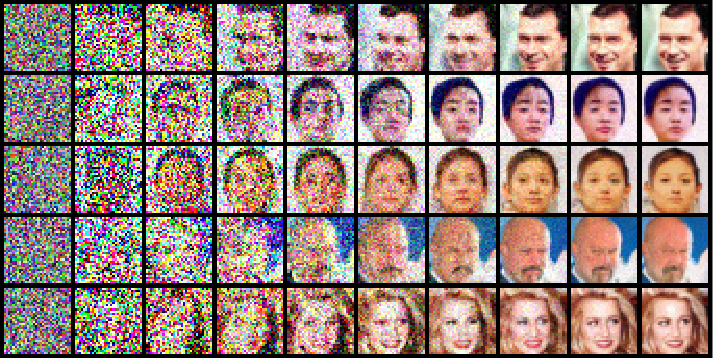
\includegraphics[height=0.18\textheight]{songermon1a.png} \\
	Denoiser = median &
	Denoiser = DCNN (generic) &
	Denoiser = DCNN (faces)
\end{tabular}
}
\end{frame}


\begin{frame}
OUTLINE\\
=======

\vfill

1. Implicit image priors by {\bf iterative denoising}\\
$\ \quad${\color{gray}($\approx$ 10min)}

2. Application to {\bf linear inverse problems}\\
$\ \quad${\color{gray}($\approx$ 5min)}

3. Colophon: implementation details\\
$\ \quad${\color{gray}($\approx$ 5min)}

\vfill

\end{frame}


% 1. iteration of denoisers
\begin{frame}%

\vfill
\begin{center}
\Huge
--1--\\Iteration of Denoisers
\end{center}
\vfill
\small
\centering
{And how each denoiser defines an implicit image prior}
\end{frame}


% 1.0 goal: understand the normalizations in K-S algorithm

% 1.1 what happens if we denoise an image iteratively?
% experiment using gaussian blur, without normalization
% experiment using gaussian blur, with normalization
% experiment using median filter, with normalization
\begin{frame}
WHAT HAPPENS IF WE DENOISE AN IMAGE ITERATIVELY?\\
================================================

Denoiser = average of 9-neighborhood

%SCRIPT plambda zero:40x40 "randu 255 *" -o f/u.png
%SCRIPT ntiply 8 f/u.png f/u8.png
%SCRIPT X() { blur square 3 ; }
%SCRIPT cat f/u.png |X| ntiply 8 - f/Xu.png
%SCRIPT cat f/u.png |X|X| ntiply 8 - f/XXu.png
%SCRIPT cat f/u.png |X|X|X| ntiply 8 - f/XXXu.png
%SCRIPT cat f/u.png |X|X|X|X|X|X|X|X|X|X| ntiply 8 - f/X10u.png

\begin{tabular}{lllll}
\includegraphics[width=0.18\linewidth]{f/u8.png}&
\only<2->{\includegraphics[width=0.18\linewidth]{f/Xu.png}}&
\only<3->{\includegraphics[width=0.18\linewidth]{f/XXu.png}}&
\only<4->{\includegraphics[width=0.18\linewidth]{f/XXXu.png}}&
\only<5->{\includegraphics[width=0.18\linewidth]{f/X10u.png}}\\
\only<1->{u} &
\only<2->{Xu} &
\only<3->{XXu} &
\only<4->{XXXu} &
\only<5->{X10u} \\
\end{tabular}

\bigskip
\small
\color{blue}
plambda zero:40x40 "randu 255 *" -o u\\
alias X="blur square 3"

\only<2->{cat u | X > Xu}$ $\\
\only<3->{cat u | X | X > XXu}$ $\\
\only<4->{cat u | X | X | X > XXXu}$ $\\
\only<5->{cat u | X|X|X|X|X|X|X|X|X|X > X10u}$ $\\


\end{frame}


\begin{frame}[noframenumbering]
WHAT HAPPENS IF WE DENOISE AN IMAGE ITERATIVELY?\\
================================================

Denoiser = median filter of 9-neighborhood

%SCRIPT plambda zero:40x40 "randu 255 *" -o f/u.png
%SCRIPT ntiply 8 f/u.png f/u8.png
%SCRIPT Z() { plambda 'x,M9' ; }
%SCRIPT cat f/u.png |Z| ntiply 8 - f/Zu.png
%SCRIPT cat f/u.png |Z|Z| ntiply 8 - f/ZZu.png
%SCRIPT cat f/u.png |Z|Z|Z| ntiply 8 - f/ZZZu.png
%SCRIPT cat f/u.png |Z|Z|Z|Z|Z|Z|Z|Z|Z|Z| ntiply 8 - f/Z10u.png

\begin{tabular}{lllll}
\includegraphics[width=0.18\linewidth]{f/u8.png}&
\only<2->{\includegraphics[width=0.18\linewidth]{f/Zu.png}}&
\only<3->{\includegraphics[width=0.18\linewidth]{f/ZZu.png}}&
\only<4->{\includegraphics[width=0.18\linewidth]{f/ZZZu.png}}&
\only<5->{\includegraphics[width=0.18\linewidth]{f/Z10u.png}}\\
\only<1->{u} &
\only<2->{Zu} &
\only<3->{ZZu} &
\only<4->{ZZZu} &
\only<5->{Z10u} \\
\end{tabular}

\bigskip
\small
\color{blue}
plambda zero:40x40 "randu 255 *" -o u\\
alias Z="plambda x,M9"

\only<2->{cat u | Z > Zu}$ $\\
\only<3->{cat u | Z | Z > ZZu}$ $\\
\only<4->{cat u | Z | Z | Z > ZZZu}$ $\\
\only<5->{cat u | Z|Z|Z|Z|Z|Z|Z|Z|Z|Z > Z10u}$ $\\


\end{frame}




%\begin{frame}
\begin{frame}[noframenumbering]
WHAT HAPPENS IF WE DENOISE AN IMAGE ITERATIVELY?\\
================================================

Denoiser = gaussian blur of~$\sigma\!=\!2$

%SCRIPT plambda zero:40x40 "randu 255 *" -o f/u.png
%SCRIPT ntiply 8 f/u.png f/u8.png
%SCRIPT Y() { blur gauss 2 ; }
%SCRIPT cat f/u.png |Y| ntiply 8 - f/Yu.png
%SCRIPT cat f/u.png |Y|Y| ntiply 8 - f/YYu.png
%SCRIPT cat f/u.png |Y|Y|Y| ntiply 8 - f/YYYu.png
%SCRIPT cat f/u.png |Y|Y|Y|Y|Y|Y|Y|Y|Y|Y| ntiply 8 - f/Y10u.png

\begin{tabular}{lllll}
\includegraphics[width=0.18\linewidth]{f/u8.png}&
\only<2->{\includegraphics[width=0.18\linewidth]{f/Yu.png}}&
\only<3->{\includegraphics[width=0.18\linewidth]{f/YYu.png}}&
\only<4->{\includegraphics[width=0.18\linewidth]{f/YYYu.png}}&
\only<5->{\includegraphics[width=0.18\linewidth]{f/Y10u.png}}\\
\only<1->{u} &
\only<2->{Yu} &
\only<3->{YYu} &
\only<4->{YYYu} &
\only<5->{Y10u} \\
\end{tabular}

\bigskip
\small
\color{blue}
plambda zero:40x40 "randu 255 *" -o u\\
alias Y="blur gauss 2"

\only<2->{cat u | Y > Yu}$ $\\
\only<3->{cat u | Y | Y > YYu}$ $\\
\only<4->{cat u | Y | Y | Y > YYYu}$ $\\
\only<5->{cat u | Y|Y|Y|Y|Y|Y|Y|Y|Y|Y > Y10u}$ $\\


\end{frame}




\begin{frame}
ITERATIVE DENOISING WITH NORMALIZATION\\
======================================

"Denoiser": gaussian blur of~$\sigma\!=\!2$ {\color{red} with normalization}

%SCRIPT plambda zero:40x40 "randu 255 *" -o f/u.png
%SCRIPT ntiply 8 f/u.png f/u8.png
%SCRIPT N() { blur gauss 2 | qauto -p 1 ; }
%SCRIPT cat f/u.png |N| ntiply 8 - f/Nu.png
%SCRIPT cat f/u.png |N|N| ntiply 8 - f/NNu.png
%SCRIPT cat f/u.png |N|N|N| ntiply 8 - f/NNNu.png
%SCRIPT cat f/u.png |N|N|N|N|N|N|N|N|N|N| ntiply 8 - f/N10u.png

\begin{tabular}{lllll}
\includegraphics[width=0.18\linewidth]{f/u8.png}&
\only<2->{\includegraphics[width=0.18\linewidth]{f/Nu.png}}&
\only<3->{\includegraphics[width=0.18\linewidth]{f/NNu.png}}&
\only<4->{\includegraphics[width=0.18\linewidth]{f/NNNu.png}}&
\only<5->{\includegraphics[width=0.18\linewidth]{f/N10u.png}}\\
\only<1->{u} &
\only<2->{Yu} &
\only<3->{YYu} &
\only<4->{YYYu} &
\only<5->{Y10u} \\
\end{tabular}

\bigskip
\small
\color{blue}
plambda zero:40x40 "randu 255 *" -o u\\
alias Y="blur gauss 2 {\color{red}\bf | qauto}"

\only<2->{cat u | Y > Yu}$ $\\
\only<3->{cat u | Y | Y > YYu}$ $\\
\only<4->{cat u | Y | Y | Y > YYYu}$ $\\
\only<5->{cat u | Y|Y|Y|Y|Y|Y|Y|Y|Y|Y > Y10u}$ $\\


\end{frame}



\begin{frame}[noframenumbering]
ITERATIVE DENOISING WITH NORMALIZATION\\
======================================

"Denoiser": median filter {\color{red} with normalization}

%SCRIPT plambda zero:40x40 "randu 255 *" -o f/u.png
%SCRIPT ntiply 8 f/u.png f/u8.png
%SCRIPT T() { plambda x,M9 | qauto -p 1 ; }
%SCRIPT cat f/u.png |T| ntiply 8 - f/Tu.png
%SCRIPT cat f/u.png |T|T| ntiply 8 - f/TTu.png
%SCRIPT cat f/u.png |T|T|T| ntiply 8 - f/TTTu.png
%SCRIPT cat f/u.png |T|T|T|T|T|T|T|T|T|T| ntiply 8 - f/T10u.png

\begin{tabular}{lllll}
\includegraphics[width=0.18\linewidth]{f/u8.png}&
\only<2->{\includegraphics[width=0.18\linewidth]{f/Tu.png}}&
\only<3->{\includegraphics[width=0.18\linewidth]{f/TTu.png}}&
\only<4->{\includegraphics[width=0.18\linewidth]{f/TTTu.png}}&
\only<5->{\includegraphics[width=0.18\linewidth]{f/T10u.png}}\\
\only<1->{u} &
\only<2->{Zu} &
\only<3->{ZZu} &
\only<4->{ZZZu} &
\only<5->{Z10u} \\
\end{tabular}

\bigskip
\small
\color{blue}
plambda zero:40x40 "randu 255 *" -o u\\
alias Z="plambda x,M9 {\color{red}\bf | qauto}"

\only<2->{cat u | Z > Zu}$ $\\
\only<3->{cat u | Z | Z > ZZu}$ $\\
\only<4->{cat u | Z | Z | Z > ZZZu}$ $\\
\only<5->{cat u | Z|Z|Z|Z|Z|Z|Z|Z|Z|Z > Z10u}$ $\\


\end{frame}

% 
\begin{frame}\small
THE SPIRIT OF A DENOISER\\
========================

Idea: each denoiser has an intrinsic ``texture'' of images that it produces by
iteration.


%gaussian=perlin

%median filter=median blobs

%SCRIPT X() { blur gauss 3 | qauto -f -p 0 ; }
%SCRIPT Y() { morsi disk5.1 median | qauto -f -p 0 ; }
%SCRIPT plambda zero:256x256 randg|X|X|X|X|X|X|X|X|X|X|qauto -p 0 - f/gX10.png
%SCRIPT plambda zero:256x256 randg|Y|Y|Y|Y|Y|Y|Y|Y|Y|Y|qauto -p 0 - f/gY10.png

\begin{tabular}{ll}
	\includegraphics[width=0.42\linewidth]{f/gX10.png}&
	\includegraphics[width=0.42\linewidth]{f/gY10.png}\\
\end{tabular}

\vfill
\small
\color{blue}
X() $\{$ blur gauss 3 | qauto ; $\}$ \\
Y() $\{$ morsi disk5.1 median | qauto ; $\}$\\
plambda zero:256x256 randg |X|X|X|X|X|X|X|X|X|X\\
plambda zero:256x256 randg |Y|Y|Y|Y|Y|Y|Y|Y|Y|Y

\end{frame}



% 1.2. review ks algorithm
\begin{frame}
OVERVIEW OF KS ALGORITHM\\
========================

\vfill
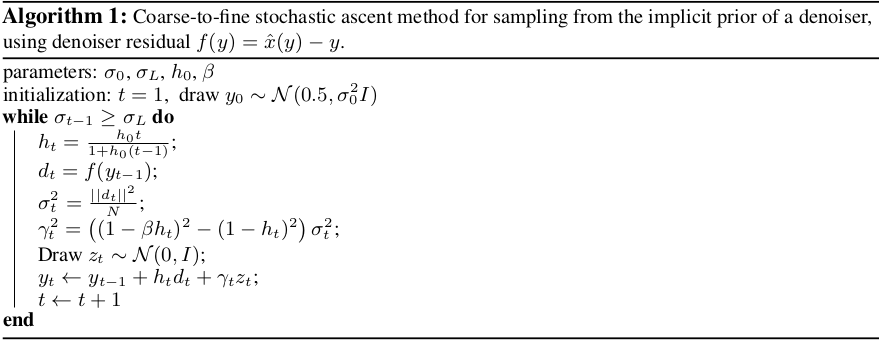
\includegraphics[width=0.9\linewidth]{ks.png}\footnotesize
\vfill
\pause
Simplified version (no jittering and all constants=1):

\color{blue}
\noindent\fbox{%
	\begin{minipage}{0.8\textwidth}
		{\bf Input:} Denoiser~$\color{red}D$,
		stepsize~$\color{darkgreen}h$, starting noise~$\sigma_0$\\
		{\bf Output:} Image~$y$\\
$ $\\
%	\parbox{0.5\textwidth}{%
$y\leftarrow\mathcal{N}(127,\sigma_0)$\\
$\mathrm{for}\ t=1,\ldots,T\ :$\\
$\phantom{mmmm}y\leftarrow y + {\color{darkgreen}h} \left({\color{red}D}(y)-y\right)$\\
$\mathrm{return}\ y$
\end{minipage}
}

\end{frame}


% 1.3. algorithm written in terms of residual denoising
% alias X='plambda ``x x,V9 rot - 1 * x +'''
% alias X='plambda ``x,M9 x - 0.9 * x +'''
% plambda zero:128x128 randu|X|X|X|X|X|X|X|X|X|X|X|X|X|X|X|X|ntiply 10|d
% cat barbara.png|X|X|X|X|X|X|X|X|X|X|X|X|X|X|X|X|ntiply 10|d
\begin{frame}
LINK WITH HEAT EQUATION\\
=======================

What is the meaning of this step?

{
\color{blue}
$\phantom{mmmm}y\leftarrow y + {\color{darkgreen}h} \left({\color{red}D}(y)-y\right)$
}
\pause

%SCRIPT blur g 3  photos/gbarbsquare.png f/gblur3.png
%SCRIPT plambda f/gblur3.png photos/gbarbsquare.png - -o f/dgblur3.npy
%SCRIPT qauto f/dgblur3.npy f/dgblur3.png
%SCRIPT plambda photos/gbarbsquare.png f/dgblur3.npy '0.7 * +' -o f/dgstep.png

\begin{tabular}{cccc}
	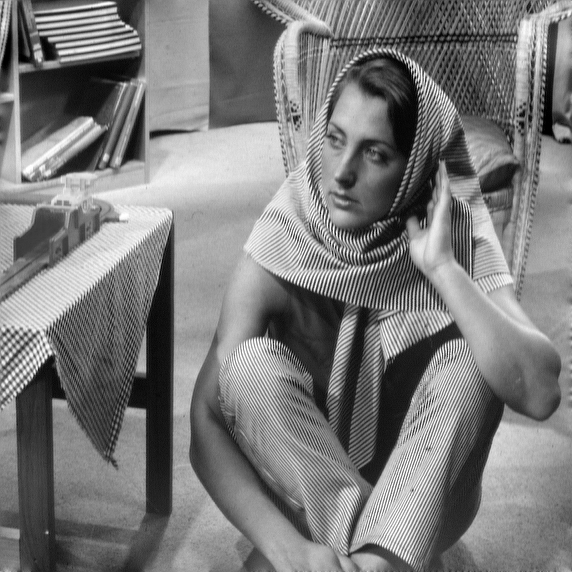
\includegraphics[width=0.23\linewidth]{photos/gbarbsquare.png}&
	\includegraphics[width=0.23\linewidth]{f/gblur3.png}&
	\includegraphics[width=0.23\linewidth]{f/dgblur3.png}&
	\includegraphics[width=0.23\linewidth]{f/dgstep.png}\\
	$\footnotesize y$ &
	$\footnotesize D(y)$ &
	$\footnotesize D(y)-y$ &
	$\footnotesize y + \frac12\left(D(y)-y\right)$
\end{tabular}

\pause
{\small
This is {\bf one step} of the numerical solution of heat equation!
}

\fbox{
$\frac{u^{n+1}-u^n}\tau=\Delta u^n$
}
\hfill
\fbox{
	$u^{n+1}=u^n+\tau\Delta u^n\color{blue} \approx u^n+\tau\left(g*u^n-u^n\right)$
}


\end{frame}

\begin{frame}[noframenumbering]
LINK WITH HEAT EQUATION\\
=======================

{\bf Proposition.}
Applying the KS iterations to the {\color{blue} gaussian blur} denoiser
computes an approixmation of the heat equation {\color{blue}
$u_t=\mathrm{div}\left(\nabla u\right)$}.

\pause

{\bf Proposition.}
Applying the KS iterations to the {\color{blue} median filter} denoiser
computes an approixmation of the mean curvature flow
{\color{blue}$u_t=\left\|\nabla u\right\|\mathrm{div}\left(\frac{\nabla
u}{\left\|\nabla u\right\|}\right)$}.

\pause

\vfill
\color{red}
What about fancier denoisers?\\
\bf You get fancier PDE!
\vfill

\end{frame}


%% 1.4. link with heat equation
%\begin{frame}
%DENOISING VS RESIDUAL DENOSING\\
%==============================
%
%
%\end{frame}
%
%
%% 1.5. further links: moisan image iterative filtering, alvarez etal
%\begin{frame}
%LINK WITH OTHER PDE\\
%===================
%
%\end{frame}


% 1.6. recall main result of alvarez etal
\begin{frame}
IMAGE PDE: GENERAL RESULTS\\
==========================

\only<1>{
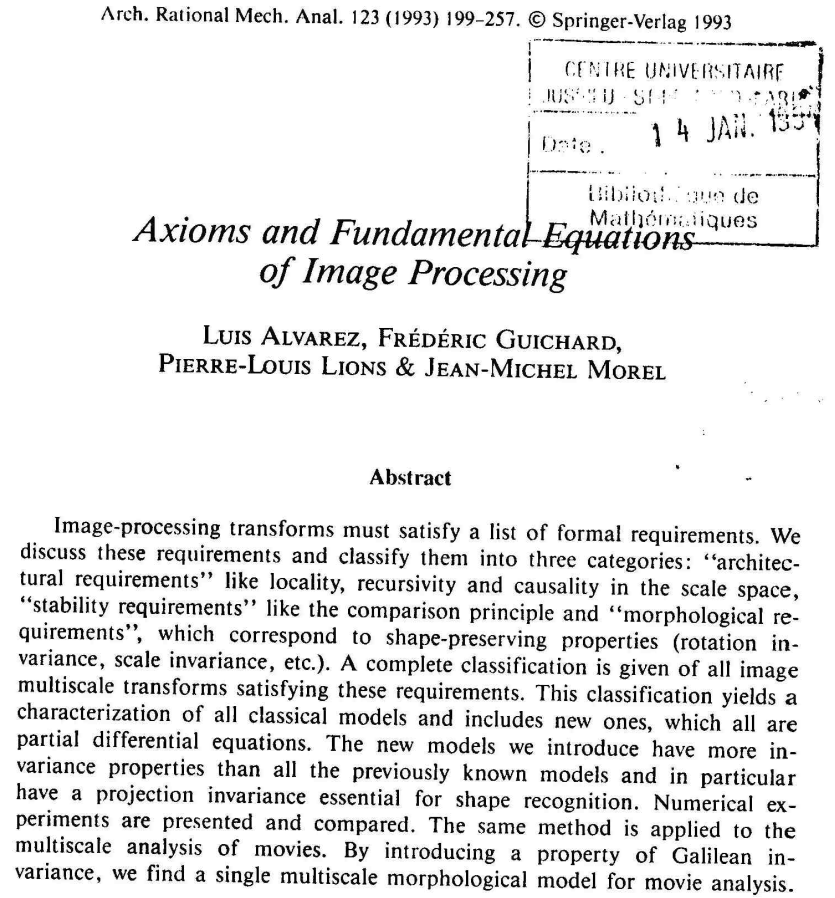
\includegraphics[width=0.49\textwidth]{photos/aglm.png}%
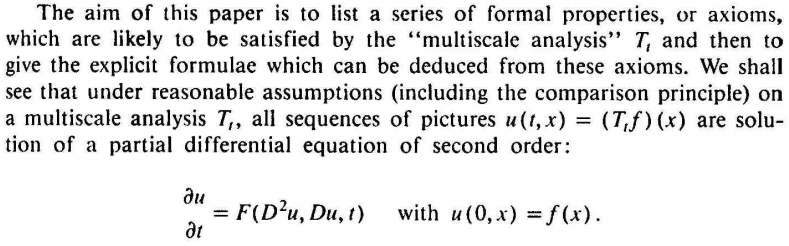
\includegraphics[width=0.49\textwidth]{photos/aglm2.png}
}\only<2>{
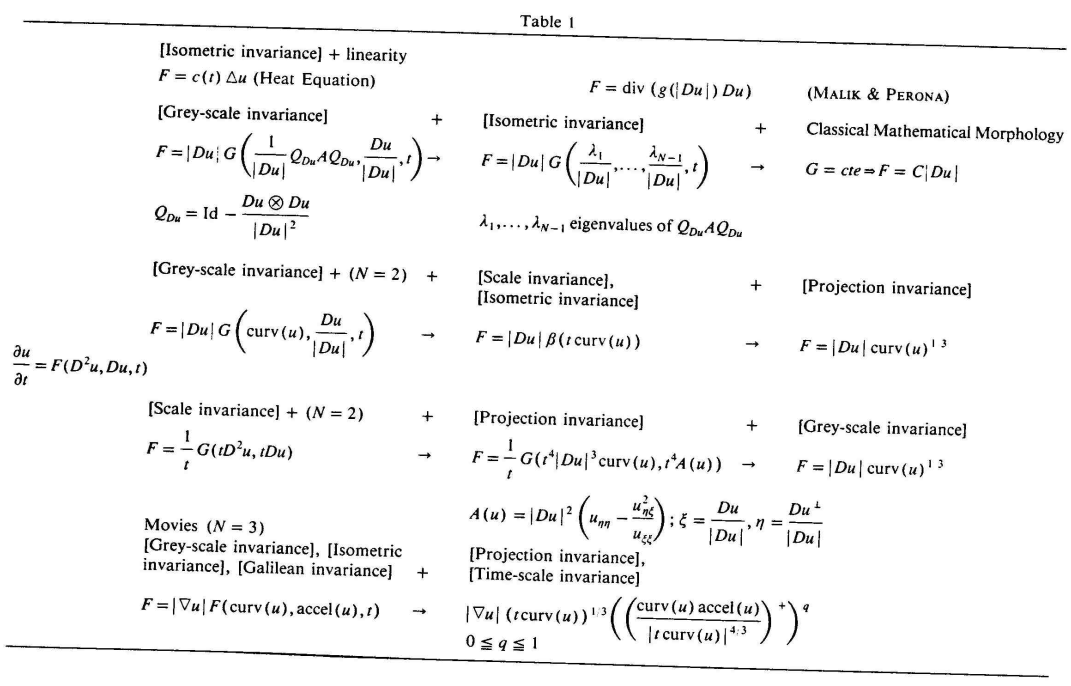
\includegraphics[width=\textwidth]{photos/aglm_table.png}%
}\only<3>{
	{\bf Conclusion:}

	Under very general assumptions on the denoiser (regularity, symmetry,
	{\color{red}locality}), the KS algorithm computes a PDE of the form
	\[
		u_t = F(D^2u, Du, t)
	\]
	\vfill
	{\bf Corrollary.}  To obtain really fancy images using KS, you
	need to use a (very) non-local denoiser.
}

\end{frame}

\begin{frame}
IMPLICIT IMAGE MODELS OF CLASSICAL DENOISERS\\
============================================

\tiny
\begin{tabular}{lll}
	
\includegraphics[width=0.31\textwidth]{out_perlin.png} &
	\includegraphics[width=0.31\textwidth]{out_mcm.png} &
	\includegraphics[width=0.31\textwidth]{out_dct.png} \\
	gausssian blur (perlin noise) &
	median filter (mcm) &
	dct denoising \\
	&&\\
	\includegraphics[width=0.31\textwidth]{out_nlm0.png} &
	\includegraphics[width=0.31\textwidth]{out_nlbayes.png} &
	\includegraphics[width=0.31\textwidth]{out_ffdnet.png} \\
	non-local means (nl diffusion) &
	non-local bayes &
	ffdnet \\
\end{tabular}
\end{frame}

\begin{frame}
FOR SOME DENOISERS, THE ALGORITHM IS TRICKY TO TUNE\\
===================================================

KS samples using the ``drunet'' denoiser

{
	\setlength{\fboxsep}{0pt}%
	\setlength{\fboxrule}{1pt}%
\begin{tabular}{lll}
	\fbox{\includegraphics[width=0.31\textwidth]{f2/out_200.png}} &
	\fbox{\includegraphics[width=0.31\textwidth]{f2/out_201.png}} &
	\fbox{\includegraphics[width=0.31\textwidth]{f2/out_211.png}} \\
	\fbox{\includegraphics[width=0.31\textwidth]{f2/out_240.png}} &
	\fbox{\includegraphics[width=0.31\textwidth]{f2/out_249.png}} &
	\fbox{\includegraphics[width=0.31\textwidth]{f2/out_251.png}} \\
\end{tabular}
}
\end{frame}


% 1.7. interpretation of other steps in KS algorithm
\begin{frame}
OTHER STEPS IN THE KS ALGORITHM\\
===============================

\vfill
\includegraphics[width=0.9\linewidth]{ks.png}\footnotesize
\vfill
\scriptsize
\color{blue}
* The step sizes~$h_t$ decrease to~$0$.

* If $\beta < 1$, gaussian noise of strength~$\gamma_t^2$ is added at each step

* $\sigma_t^2$ is the variance of the previous residual (used only for~$\gamma_t$)
\vfill
\end{frame}


%% 1.8. experiments with various versions of parameters, classical denoisers
%\begin{frame}
%SOME EXPERIMENTS WITH VARIOUS PARAMETERS\\
%========================================
%
%\end{frame}
%
%
%% 1.9. slightly fancier denoisers
%\begin{frame}
%SLIGHTLY FANCIER DENOISERS\\
%==========================
%
%\end{frame}


% 1.10. the ks notebook
\begin{frame}
FROM THE KS NOTEBOOK\\
====================

The KS article includes a color denoiser named {\bf BF-CNN}.  Below are some synthesis results.


\vfill
\includegraphics[width=\textwidth]{f2/ksdemo1.png}
\includegraphics[width=\textwidth]{f2/ksdemo2.png}
\includegraphics[width=\textwidth]{f2/ksdemo3.png}
\includegraphics[width=\textwidth]{f2/ksdemo4.png}
\vfill

\scriptsize
Notebook to try:\\
{\color{blue}\url{
https://github.com/LabForComputationalVision/universal_inverse_problem
}}
\end{frame}

\begin{frame}
FROM THE KS NOTEBOOK\\
====================

More examples using {\bf BF-CNN}

\vfill
\begin{tabular}{lll}
	\includegraphics[width=0.31\textwidth]{f2/untitled.png}&
	\includegraphics[width=0.31\textwidth]{f2/untitled2.png}&
	\includegraphics[width=0.31\textwidth]{f2/untitled3.png}\\
	\includegraphics[width=0.31\textwidth]{f2/untitled4.png}&
	\includegraphics[width=0.31\textwidth]{f2/untitled5.png}&
	\includegraphics[width=0.31\textwidth]{f2/untitled6.png}\\
\end{tabular}


\scriptsize
Notebook to try:\\
{\color{blue}\url{
https://github.com/LabForComputationalVision/universal_inverse_problem
}}
\end{frame}

\begin{frame}
INTERPRETATION\\
==============

\vfill
\includegraphics[width=\textwidth]{f2/ksfig.png}

\end{frame}






% 2. linear inverse problems
\begin{frame}%

\vfill
\begin{center}
\Huge
--2--\\Linear Inverse Problems
\end{center}
\vfill
\small
\centering
{And how can we solve them using a denoiser}
\end{frame}



% 2.0. linear inverse problems: definition
\begin{frame}
LINEAR INVERSE PROBLEMS : DEFINITION\\
====================================

It's just a problem with linear constraints:

$\qquad\min E(x)$\\
$\qquad\mathrm{s.t.}\ {\color{red}M}x=t$

\vfill
Examples:

{\bf Inpainting:}\\
$M=$ value of the pixels on a part of the image.

{\bf Super-resolution:} $M=$ zoom-out operator.

{\bf Spectral inpainting:} $M=$ fix a part of the spectrum

\end{frame}

\begin{frame}
LINEAR INVERSE PROBLEMS : INTERPRETATION\\
========================================

\begin{tabular}{ll}
	\includegraphics[width=0.47\linewidth]{f2/ksfig3.png}&
	\includegraphics[width=0.47\linewidth]{f2/ksfig4.png}\\
	base KS &
	project to M at each iteration
\end{tabular}

\end{frame}


%% 2.1. examples of linv problems: inpainting, spatial zoom-in, spectral zoom-in
%\begin{frame}
%EXAMPLES OF LINEAR INVERSE PROBLEMS\\
%===================================
%
%\end{frame}

% 2.2. see the modified algorithm
\begin{frame}
MODIFIED KS ALGORITHM\\
=====================

\includegraphics[width=\linewidth]{ks2.png}

\end{frame}

% 2.3. link with laplace inpainting
\begin{frame}
EXAMPLES\\
========

\only<1>{\includegraphics[width=\linewidth]{f2/inp1.png}}
\only<2>{\includegraphics[width=\linewidth]{f2/inp2.png}}
\only<3>{\includegraphics[width=\linewidth]{f2/inp3.png}}
\only<4>{\includegraphics[width=\linewidth]{f2/inp4.png}}

\end{frame}

% 2.4. link with tv inpainting
\begin{frame}
LINK WITH PDE INPAINTING\\
========================

Denoiser=gaussian $\Longrightarrow$ harmonic inpainting

denoiser=meduian $\Longrightarrow$ TV inpainting

\end{frame}

%% 2.5. examples with fancier denoisers
%\begin{frame}
%EXAMPLES WITH FANCIER DENOISERS\\
%===============================
%
%\end{frame}



% 2. linear inverse problems
\begin{frame}%

\vfill
\begin{center}
\Huge
--3--\\Colophon
\end{center}
\vfill
\small
\centering
{implementation details}
\end{frame}


% 3.0. colophon: implementation details
% 3.1. show the ks source code (core algorithm)
\begin{frame}
SOURCE CODE OF THE KS ALGORITHM: {\bf CORE FUNCTION}\\
==============================================

\includegraphics[width=\linewidth]{f2/kscode.png}

\end{frame}

% 3.2. show the ks source code (main function, with denoiser selection)
\begin{frame}
SOURCE CODE OF THE KS ALGORITHM: {\bf DENOISER SELECTION}\\
===================================================

\includegraphics[width=\linewidth]{f2/kscode2.png}

\end{frame}

% 3.3. pip install ipol
\begin{frame}
PIP INSTALL IPOL\\
================

%see local ipol run
\includegraphics[height=0.9\textheight]{clipolcollab.png}

\end{frame}

%% 3.4. local ipol run
%\begin{frame}
%a\\
%=========================================
%
%\end{frame}

% 3.5. idl and their shenanigans
\begin{frame}
IPOL DESCRIPTION LANGUAGE EXAMPLES\\
==================================

(I don't want to show this, yet...)

\end{frame}


% ending:
% k-s photos and links to presentations (IHES/simmons)
%
% Zahra Kadkhodaie
% Flatiron-Wide Machine Learning
% Flatiron Institute, June 2023
% https://www.youtube.com/watch?v=24IukBNPJLw
%
% Eero Simoncelli
% Photographic Image Priors in the Era of Machine Learning
% IHES, April 2023 (in honor of Mallat's birthday)
% https://www.youtube.com/watch?v=OiZFsn0_rjk
\begin{frame}
REFERENCES\\
==========

\vfill

\begin{tabular}{ll}
	\includegraphics[width=0.4\linewidth]{photos/kadkhodaie2.jpg}&
	\includegraphics[width=0.4\linewidth]{photos/simoncelli2.jpg}\\
	Zahra Kadkhodaie & Eero Simoncelli \\
\end{tabular}

\vfill

\scriptsize

% Zahra Kadkhodaie
%Flatiron-Wide Machine Learning\\
{\bf Solving Linear Inverse Problems Using the Prior Implicit in a Denoiser}\\
Flatiron Institute, June 2023\\
{\color{blue}\url{https://www.youtube.com/watch?v=24IukBNPJLw}}

% Eero Simoncelli
{\bf Photographic Image Priors in the Era of Machine Learning}\\
IHES, April 2023 (in honor of Mallat's birthday)\\
{\color{blue}\url{https://www.youtube.com/watch?v=OiZFsn0_rjk}}\\

\vfill

\end{frame}




\end{document}

%\begin{frame}
%IMPLICIT IMAGE MODELS OF CLASSICAL DENOISERS\hfill{\footnotesize{\color{gray}mnhrdt}}\\
%============================================
%
%\small
%Any denoiser contains an ``implicit image prior''.\\
%How can we can extract images from it?
%
%{\color{gray}Kadkhodaie-Simoncelli 2021}\\
%\includegraphics[width=0.7\linewidth]{ks.png}
%
%%\vfill
%{\bf Demo: } Bring your own denoiser for this algorithm
%
%%\vfill
%\tiny
%\begin{tabular}{lll}
%	\includegraphics[height=0.18\textheight]{somiters3b.png} &
%	\includegraphics[height=0.18\textheight]{songermon1b.png} &
%	\includegraphics[height=0.18\textheight]{songermon1a.png} \\
%	Denoiser = median &
%	Denoiser = DCNN (generic) &
%	Denoiser = DCNN (faces)
%\end{tabular}
%
%\end{frame}
%
%\begin{frame}
%IMPLICIT IMAGE MODELS OF CLASSICAL DENOISERS
%============================================
%
%%Computed with current code:
%%Particular cases of Kadkhodaie-Simoncelli dynamics:
%
%\tiny
%\begin{tabular}{lll}
%	\includegraphics[width=0.31\textwidth]{out_perlin.png} &
%	\includegraphics[width=0.31\textwidth]{out_mcm.png} &
%	\includegraphics[width=0.31\textwidth]{out_dct.png} \\
%	gausssian blur (perlin noise) &
%	median filter (mcm) &
%	dct denoising \\
%	&&\\
%	\includegraphics[width=0.31\textwidth]{out_nlm0.png} &
%	\includegraphics[width=0.31\textwidth]{out_nlbayes.png} &
%	\includegraphics[width=0.31\textwidth]{out_ffdnet.png} \\
%	non-local means (nl diffusion) &
%	non-local bayes &
%	ffdnet \\
%\end{tabular}
%
%\end{frame}
%
%\begin{frame}
%SUBPRODUCT: PYTHON INTERFACE TO IPOL ALGORITHMS
%===============================================
%
%\includegraphics[height=0.9\textheight]{clipolcollab.png}
%\end{frame}
%
%
%\end{document}


% vim:sw=2 ts=2 spell spelllang=fr:
